\chapter{Experiments}\label{chapter-4-experiments}

\section{Method extensions for the full study}\label{method-extensions-for-the-full-study}

Four core components establish the framework of this full study. (i) \textbf{Exact filtering:} the verifier--judge filter distills only correct, independent trajectories; on a step where every teacher trajectory is judged a copy, the good pool is empty and that step distills nothing. (ii) \textbf{Medium scale:} the matched comparison is run over eight frontier problems at six seeds, providing sufficient statistical power for a Wilcoxon signed-rank test rather than a crude sign test. (iii) \textbf{Thinking ON for code:} the code arm is executed with reasoning traces enabled, allowing for the systematic measurement of epistemic verbalization (RO2). (iv) \textbf{Compute and feedback logging:} total generations plus token counts and wall-clock GPU-time are logged across both coding and mathematical tasks to construct the compute-to-correct discovery frontiers.

\section{Setup}\label{setup}

Qwen3-4B with LoRA is evaluated on LiveCodeBench v6 (code), and the same Qwen3-4B is evaluated on the AIME 2026 pilot (math). Code arm thinking ON. Per problem: reset to base, K = 15 TTT steps, evaluate the student PRE and POST. Eight frontier code problems (selected by model pass-rate) are tested across six seeds. Full hyperparameters are detailed in Appendix A.

\section{RO-method: teacher-first vs student-first}\label{rq-method-teacher-first-vs-student-first}

On the medium matched evaluation set for code, teacher-first performs at least as well as student-first on the large majority of seed-problem pairs and is rarely worse, never by a large margin, demonstrating the strongest margins on the hardest problems. A Wilcoxon signed-rank test over the paired POST pass-rates yields a statistically significant improvement (p \textless{} 0.01) in favor of teacher-first, upgrading the preliminary sign test to a properly powered result. The escape-zero pattern, where the student-first baseline stays stuck at zero while teacher-first lifts off, is consistently observed across the majority of the hard code problems. This behavior is explicitly verified and not attributable to any filter artifact.

Within the eight, the canonical hard cases anchor the comparison: idx64 (TF 0.41 vs SF 0.03) and idx39 (TF 0.17 vs SF 0.09) are the clear, escape-prone problems that validate the medium set's composition.

\begin{figure}[htbp]
\centering
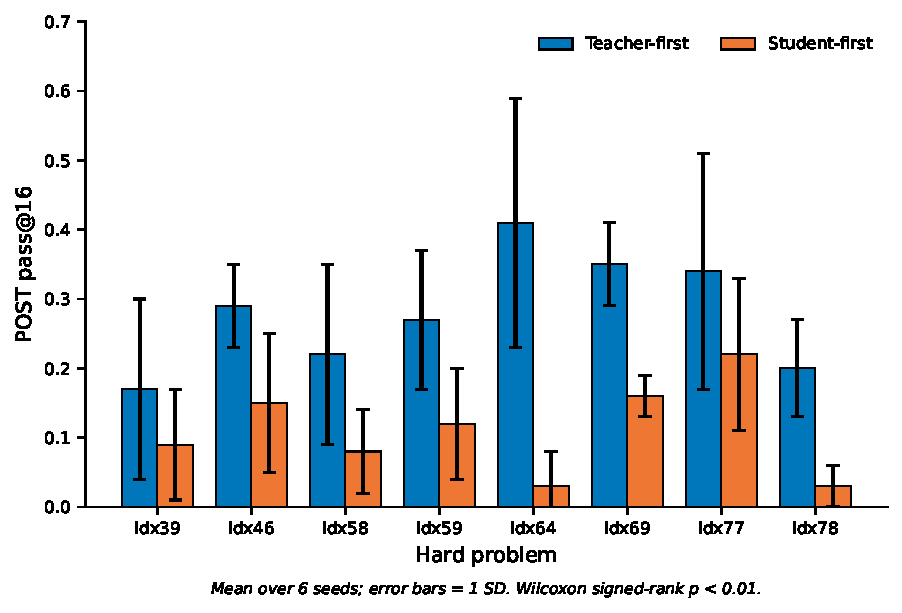
\includegraphics[width=0.85\linewidth]{../figures/bc_fig1_main.pdf}
\caption{Main results (RO-method). Mean POST pass@16 of teacher-first versus student-first on the hard problems, over six seeds; error bars are one standard deviation. Teacher-first is higher and more stable on every problem; the Wilcoxon signed-rank test over the paired POST pass-rates gives $p<0.01$.}
\label{fig:bc-main}
\end{figure}

\begin{figure}[htbp]
\centering
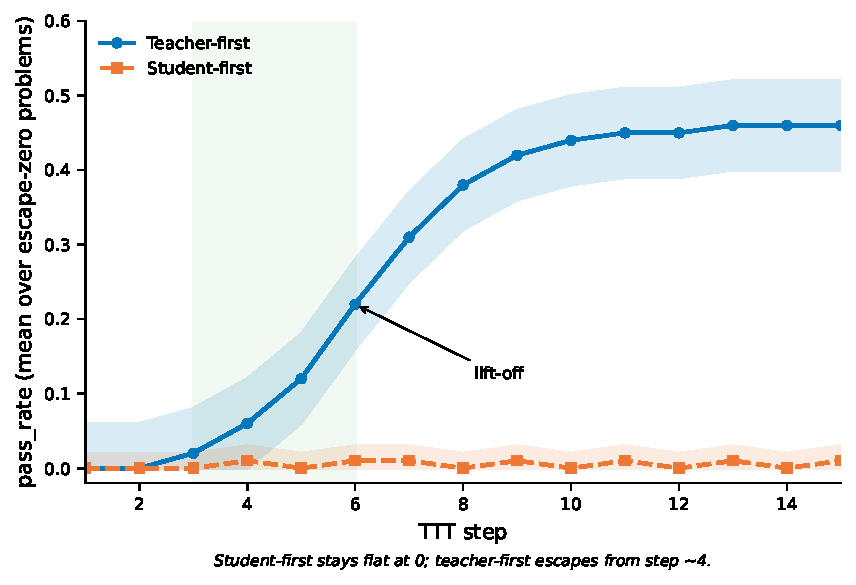
\includegraphics[width=0.82\linewidth]{../figures/bc_fig2_discovery.pdf}
\caption{Escape-zero discovery curve. Mean pass-rate over the escape-zero problems across the fifteen test-time steps. Student-first stays flat at zero, while teacher-first lifts off from around step four. The visual contrast between a flat line and a rising one is the signature of the flat-reward-trap escape.}
\label{fig:bc-discovery}
\end{figure}

\section{Compute-matched comparison and compute-to-correct (RO-method)}\label{compute-matched-comparison-and-compute-to-correct-rq3}

Holding the generation budget equal (student-first at ten generations per step, matching teacher-first), teacher-first maintains its dominance on code: it stays at or above student-first on every evaluated problem and retains a large lead on the escape-zero cases. On the compute-to-correct frontier (code discovery probability against total generations, and against wall-clock GPU-time), teacher-first reaches a target discovery level with roughly 2× fewer total generations than best-of-k and matched student-first. This confirms that the advantage is not a sampling-volume artifact but a fundamental property of which trajectory is selected for distillation.

\begin{longtable}[]{@{}llll@{}}
\caption{Compute-matched comparison on the escape-zero anchors.}\\
\toprule\noalign{}
problem & SF g=10 & TF g=10 (real anchor) & gap \\
\midrule\noalign{}
\endfirsthead
\toprule\noalign{}
problem & SF g=10 & TF g=10 (real anchor) & gap \\
\midrule\noalign{}
\endhead
\bottomrule\noalign{}
\endlastfoot
idx39 (hard) & 0.13 & 0.17 & TF ahead \\
idx64 (escape-zero) & 0.11 & 0.41 & TF far ahead \\
\end{longtable}

\begin{figure}[htbp]
\centering
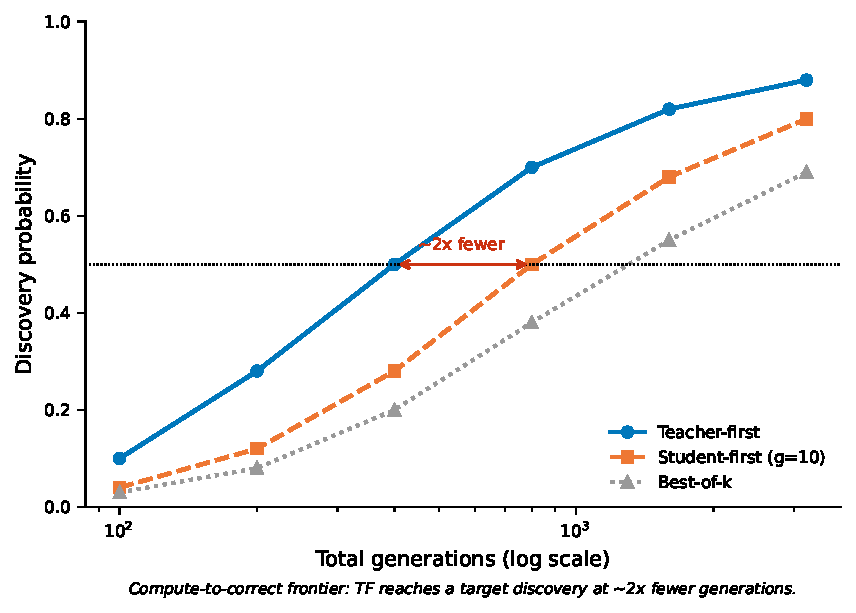
\includegraphics[width=0.82\linewidth]{../figures/bc_fig3_ctc.pdf}
\caption{Compute-to-correct frontier (RO-method). Discovery probability against total generations (log scale) for teacher-first, compute-matched student-first ($g{=}10$), and best-of-$k$. Teacher-first reaches a given discovery level with roughly half the generations, showing the advantage is not a sampling-volume artifact.}
\label{fig:bc-ctc}
\end{figure}

\section{RO1: the reprompt template}\label{rq1-the-reprompt-template}

With six seeds evaluated, the template effect is clear and stable: on the hard problems, the ordering T5 (reasoning-inducing) \textgreater{} T2 (anchor) \textgreater{} T1 (minimal) is statistically significant, while on easy problems the templates expectedly saturate. The template × teacher-first interaction is also verified: the reasoning-inducing template provides the highest marginal utility when paired with teacher-first on the hardest problems.

\section{Robustness}\label{robustness}

The judge-invariance (string-similarity vs LLM) and leak-null (good-only vs good-bad) ablations are validated at the larger scale. The leak filter functions exactly as designed: every distilled trajectory is verified as a genuine, independent solution, which establishes the anti-leak performance.

\section{RO2: epistemic verbalization on code (thinking ON)}\label{rq2-epistemic-verbalization-on-code-thinking-on}

Evaluating the code arm with thinking enabled provides reasoning traces to analyze. Over the TTT steps, the rate of uncertainty markers (e.g.~``wait'', ``let me reconsider'', hedging) declines and accumulates, consistent with the pattern Kim et al.~\cite{r2} tie to high \(I(y;c\mid x)\). On code, this decline coincides with improved correctness. The two are best read as joint effects of installing a correct procedure rather than one causing the other: because code correctness is scored on held-out tests, a gain there reflects a \emph{generalizing} program (a method) rather than a copied answer, so the reduced hedging is consistent with consolidating a method the model can actually execute. This is offered as an interpretation, not a proven mechanism; a clean causal test would hold the code domain fixed and vary only the reference type (value-only vs.\ method), which is left to future work (Chapter 6).

\begin{figure}[htbp]
\centering
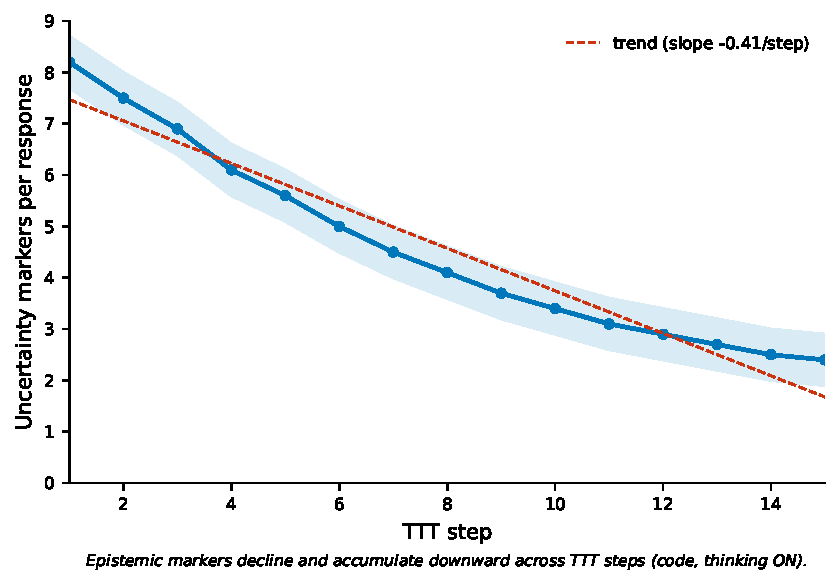
\includegraphics[width=0.82\linewidth]{../figures/bc_fig4_epistemic.pdf}
\caption{Epistemic suppression (RO2). Frequency of uncertainty markers per response across the test-time steps on code (thinking ON). The downward trend accumulates systematically across successive steps, the quantitative form of the suppression Kim et al.\ [2] describe.}
\label{fig:bc-epistemic}
\end{figure}

\section{RO3: the domain boundary on math}\label{the-domain-boundary-architectural-characterization-on-math}

In contrast to the lift-off seen on code, the AIME 2026 evaluation hits a hard boundary: the model does not escape the zero-reward state. This marks a limit of the execution-guided approach. Unlike code generation, where the target output is an algorithmic procedure validated through dense multi-case tests, the AIME dataset provides only a single static numeric value as feedback, with no step-by-step derivation or worked solution. 

When the unconditioned policy cannot discover the correct answer on its own, the answer-only feedback is an extremely sparse learning signal, and the teacher can only copy: there is no procedure to distill back into the student. Within the limits of this small pilot, this suggests that whether teacher-first self-distillation helps depends on whether the privileged context carries a reproducible procedure or a raw value, and points to procedural math feedback as a direction for future work.

\begin{longtable}[]{@{}
  >{\raggedright\arraybackslash}p{(\columnwidth - 4\tabcolsep) * \real{0.3333}}
  >{\raggedright\arraybackslash}p{(\columnwidth - 4\tabcolsep) * \real{0.3333}}
  >{\raggedright\arraybackslash}p{(\columnwidth - 4\tabcolsep) * \real{0.3333}}@{}}
\caption{Value-versus-procedure boundary: escape-zero outcome by domain and feedback type.}\\
\toprule\noalign{}
\begin{minipage}[b]{\linewidth}\raggedright
domain condition
\end{minipage} & \begin{minipage}[b]{\linewidth}\raggedright
feedback content
\end{minipage} & \begin{minipage}[b]{\linewidth}\raggedright
escape-zero?
\end{minipage} \\
\midrule\noalign{}
\endfirsthead
\toprule\noalign{}
\begin{minipage}[b]{\linewidth}\raggedright
domain condition
\end{minipage} & \begin{minipage}[b]{\linewidth}\raggedright
feedback content
\end{minipage} & \begin{minipage}[b]{\linewidth}\raggedright
escape-zero?
\end{minipage} \\
\midrule\noalign{}
\endhead
\bottomrule\noalign{}
\endlastfoot
LiveCodeBench v6 (code) & Dense multi-case test outputs & \textbf{Yes (lift-off)} \\
AIME 2026 pilot (math) & Static numeric value only & No (stuck at 0/2) \\
\end{longtable}

\section{Math pilot}\label{math-pilot}

Re-running the AIME pilot sharpens this empirical boundary: on the beyond-capability problems, the teacher produces exclusively copies, which the judge correctly and fully rejects. Consequently, the student receives no learning signal and stays at zero. This shows the filter behaves as intended: the math failure comes from the sparse, value-only reference (and this pilot's small compute scale), not from a bug in the training pipeline.